\documentclass[border=6pt]{standalone}
\usepackage{times}
\usepackage{pgfplots}
\pgfplotsset{compat=1.18}
\begin{document}
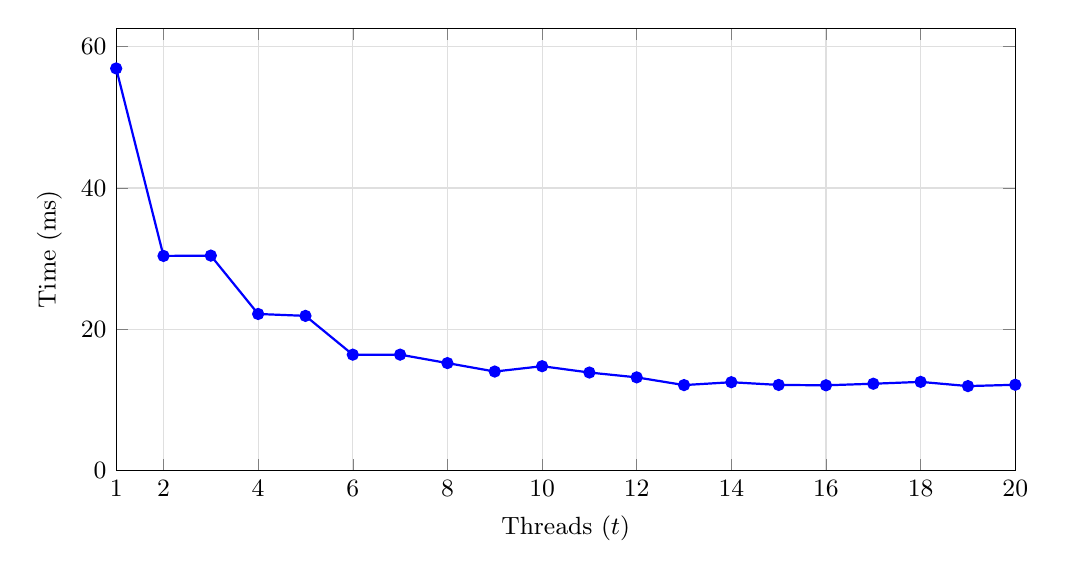
\begin{tikzpicture}
\begin{axis}[width=13cm,height=7.2cm,
xlabel={Threads ($t$)},ylabel={Time (ms)},
xmin=1,xmax=20,xtick={1,2,4,6,8,10,12,14,16,18,20},
ymin=0,grid=both,major grid style={gray!25},minor grid style={gray!10},
tick label style={font=\small},label style={font=\small},
scaled y ticks=false,/pgf/number format/1000 sep={}]
\addplot[blue,thick,mark=*,mark size=1.8pt] coordinates {
(1, 56.923203)
(2, 30.385435)
(3, 30.432386)
(4, 22.169894)
(5, 21.902259)
(6, 16.41253)
(7, 16.414411)
(8, 15.218563)
(9, 14.021936)
(10, 14.779086)
(11, 13.881864)
(12, 13.198704)
(13, 12.105628)
(14, 12.511484)
(15, 12.125598)
(16, 12.075057)
(17, 12.297321)
(18, 12.560284)
(19, 11.962966)
(20, 12.149067)
};
\end{axis}
\end{tikzpicture}
\end{document}
